\documentclass[letterpaper,12pt]{article}

\usepackage[margin=1.0in]{geometry}
\usepackage{multirow}
\usepackage{tikz}
\usepackage{amsmath}

\usetikzlibrary{shapes.geometric, arrows, fit}

\newcommand{\botname}{\textit{The Comet Cannon}}
\newcommand{\specialcell}[2][c]{\begin{tabular}[#1]{@{}c@{}}#2\end{tabular}}
\newcommand{\xxx}[1]{{\color{red}\bf #1}}
\newcommand{\AxisRotator}[1][rotate=0]{\tikz [x=0.25cm,y=0.60cm,line width=.2ex,-stealth,#1] \draw (0,0) arc (-150:150:1 and 1);}

\begin{document}

\title{T-Shirt Cannon Overview}
\author{Hazen Eckert \hspace{3mm} Omar Hasan \hspace{3mm} Ryan Marcotte \hspace{3mm} Ridhwaan Rahman}
\date{}
\maketitle

\section{System Overview}

\begin{figure}[h!]
  \centering
  \tikzstyle{block} = [rectangle, ultra thick, rounded corners, minimum width=2cm, minimum height=1cm,text centered, draw=black]
  \tikzstyle{dcvolt} = [solid, ultra thick, red];
  \tikzstyle{signal} = [solid, ultra thick, ->, >=stealth];

  \begin{tikzpicture}
    %\draw[help lines] (-6, -12) grid (12,1);
    \node (circuitbreaker) [block, align=center] {\textbf{Circuit}\\\textbf{Breaker}};
    \node (boost) [block, align=center, below of=circuitbreaker, xshift=-4cm, yshift=-2cm] {\textbf{Boost}\\\textbf{Converter}};
    \node (buck) [block, align=center, right of=boost, xshift=7cm] {\textbf{Buck}\\\textbf{Converter}};
    \node (mcu) [block, below of=buck, yshift=-1.25cm] {\textbf{MCU}};
    \node (triggersolenoid) [block, align=center, below of=boost, yshift=-3.5cm, xshift=-1.5cm] {\textbf{Trigger}\\\textbf{Solenoid}};
    \node (pressuresolenoid) [block, align=center, right of=triggersolenoid, xshift=2cm] {\textbf{Pressure}\\\textbf{Solenoid}};
    \node (encoders) [block, right of=pressuresolenoid, xshift=2cm] {\textbf{Encoders}};
    \node (pressuresensor) [block, align=center, right of=encoders, xshift=2cm] {\textbf{Pressure}\\\textbf{Sensor}};
    \node (camera) [block, align=center, right of=pressuresensor, xshift=2cm] {\textbf{Camera}\\\textbf{Module}};
    \node (esc) [block, right of=camera, xshift=2cm] {\textbf{ESC}};
    \node (motors) [block, below of=esc, xshift=-4.5cm, yshift=-1cm] {\textbf{Motors}};

    \draw [dcvolt] (circuitbreaker.north) -- +(0,0.5) node[anchor=south] {\textbf{+12V}};
    \draw [dcvolt] (circuitbreaker.south) -- +(0,-0.9) node[anchor=west, yshift=0.5cm] {\textbf{+12V}};
    \draw [dcvolt] (boost.north) -- +(0,1) -| +(4,1) node {};
    \draw [dcvolt] (buck.north) -- +(0,1) -| +(-4,1) node {};
    \draw [dcvolt] (esc.north) -- +(0,5.55) -| +(-5.5,5.55) node {};
    \draw [dcvolt] (buck.south) -- node[anchor=west, yshift=0.2cm] {\textbf{+5V}} (mcu.north);
    \draw [dcvolt] (encoders.north) -- +(0,2.7) -| +(3.5,2.7) node {};
    \draw [dcvolt] (pressuresensor.north) -- +(0,0.2) -| +(-3,0.2) node {};
    \draw [dcvolt] (camera.north) -- +(0,2.65) -| +(-2.5,2.65) node{};
    \draw [dcvolt] (boost.south) -- +(0,-1) node[anchor=west, yshift=0.5cm] {\textbf{+24V}};
    \draw [dcvolt] (triggersolenoid.north) -- +(0,2.4) -| +(1.5,2.4) node {};
    \draw [dcvolt] (pressuresolenoid.north) -- +(0,2.4) -| +(-1.5,2.4) node {};
    \draw [signal] (mcu.300) -- +(0,-1) -| +(0.7,-1) -| +(0.7,-1.75) -| (pressuresensor.east) -- ++(180:1pt);
    \draw [signal] (mcu.320) -- +(0,-0.8) -| +(3.5,-0.8) -| +(3.5,-1.75) -| (esc.west) -- ++(0:1pt);
    \draw [signal] (mcu.south) -- +(0,-0.8) -| +(-2,-0.8) -| +(-2,-1.75) -| (encoders.east) -- ++(180:1pt);
    \draw [signal] (mcu.240) -- +(0,-0.6) -| +(-4.8,-0.6) -| +(-4.8,-1.75) -| (pressuresolenoid.east) -- ++(180:1pt);
    \draw [signal] (mcu.220) -- +(0,-0.4) -| +(-7.4,-0.4) -| +(-7.4,-1.75) -| (triggersolenoid.east) -- ++(180:1pt);
    \draw [signal] (esc.south) -- +(0,-1.5) -| (motors.east) -- ++(180:1pt);
    \draw [signal] (motors.west) -- +(-3.5,0) -| (encoders.south);
  \end{tikzpicture}
  \caption{Electrical System Diagram}
  \label{fig:e_system}
\end{figure}

\begin{figure}[h!]
  \centering

  \tikzstyle{block} = [rectangle, rounded corners, minimum width=3cm, minimum height=2cm,text centered, draw=black]
\tikzstyle{container} = [draw, rectangle, rounded corners, dashed, text width=11em, inner sep=3.5em]
  \tikzstyle{arrow} = [thick, ->, >=latex]
  \begin{tikzpicture}[node distance=2cm]
    \node (input) [align=center, xshift=-1cm] {User\\Inputs};
    \node (output) [right of=input, align=center] {Video\\Display};
    \node (computer) [block, yshift=-2cm] {Computer};
    \node (ar9331) [block, right of=computer, xshift=9cm, yshift=-2cm, align=center] {Atheros\\AR9331};
    \node (atmega) [block, below of=ar9331, yshift=-2cm, align=center] {Arduino\\ATmega32u4};
    \node (rpi) [block, right of=computer, above of=ar9331, xshift=-2cm, yshift=2cm] {Raspberry Pi};

    \node (yun) [container, fit=(atmega) (ar9331)] {};
    \node (yun_text) [yshift=-0.3cm] at (yun.north) {Yun};

    \draw [arrow] (computer.336) -- node[anchor=east, align=center, yshift=-5mm] {Velocity\\Commands} (ar9331.188);
    \draw [arrow] (ar9331.172) -- node[anchor=west, align=center, xshift=-12mm, yshift=5mm] {Status Updates} (computer.352);
    \draw [arrow] (ar9331.240) -- node[anchor=east, align=center] {GPIO\\Commands} (atmega.120);
    \draw [arrow] (atmega.60) -- node[anchor=west, align=center] {Sensor\\Readings} (ar9331.300);
    \draw [arrow] (rpi.172) -- node[anchor=east, align=center, yshift=5mm] {Video\\Stream} (computer.24);
    \draw [arrow] (computer.8) -- node[anchor=west, align=center, xshift=-12mm, yshift=-5mm] {Video Commands} (rpi.188);
    \draw [arrow] (input) -- (computer.134);
    \draw [arrow] (computer.46) -- (output);
  \end{tikzpicture}
  \caption{System Overview}
  \label{fig:system_diagram}
\end{figure}

\subsection{Computer}
\subsection{AR9331}

\subsection{Serial Communication}
\label{sec:ar9331_serial_com}
\noindent The AR9331 and ATMega32U4 communicate via serial. To do this, we open the proper serial device (\texttt{/dev/ttyATH0}) and use the straightforward \texttt{write()} command. No further configuration of the serial device is necessary.


\subsubsection{Velocity Kinematics}
\label{sec:ar9331_vel_kin}

\noindent In order to command a desired robot velocity,
\begin{math}
  v=
  \begin{bmatrix}
    v_x \\
    v_y \\
    \omega_z
  \end{bmatrix}
\end{math}
, we calculate the wheel velocities as shown in Equations \ref{eq:rw_to_v}-\ref{eq:v_wheel_4}, according to Figure \ref{fig:robot_top_view}.

\begin{figure}[h!]
  \centering

  \tikzstyle{robot} = [rectangle, minimum width=3cm, minimum height=4cm,text centered, draw=black]
  \tikzstyle{wheel} = [rectangle, minimum width=5mm, minimum height=1cm, draw=black]
  \tikzstyle{arrow} = [thick, ->, >=latex]
  \tikzstyle{dist} = [thick, <->, >=|]

  \begin{tikzpicture}
    \node (robot) [robot] {};
    \node (wheel 1) [wheel, left of=robot, xshift=-7.5mm, yshift=1cm] {0};
    \node (wheel 2) [wheel, right of=robot, xshift=7.5mm, yshift=1cm] {1};
    \node (wheel 3) [wheel, right of=robot, xshift=7.5mm, yshift=-1cm] {2};
    \node (wheel 4) [wheel, left of=robot, xshift=-7.5mm, yshift=-1cm] {3};

    \draw [arrow] (0,0) -- node[anchor=north, xshift=-4mm] {y} (-1,0);
    \draw [arrow] (0,0) -- node[anchor=west, yshift=5mm] {x} (0,1);
    \draw (0,0)  -- (0,0) node[xshift=2.8mm] {\AxisRotator[x=0.3cm,y=0.3cm,->,rotate=-90,black] $\omega_z$};
    \draw [dist] (0,2.3) -- node[anchor=south] {$l_1$} (1.8,2.3);
    \draw [dist] (0.03,2.3) -- node[anchor=south] {$l_1$} (-1.8,2.3);
    \draw [dist] (0,-2.3) -- node[anchor=north] {$l_1$} (1.8,-2.3);
    \draw [dist] (0.03,-2.3) -- node[anchor=north] {$l_1$} (-1.8,-2.3);
    \draw [dist] (2.3,0) -- node[anchor=west] {$l_2$} (2.3, 1);
    \draw [dist] (2.3,0.03) -- node[anchor=west] {$l_2$} (2.3, -1);
    \draw [dist] (-2.3,0) -- node[anchor=east] {$l_2$} (-2.3, 1);
    \draw [dist] (-2.3,0.03) -- node[anchor=east] {$l_2$} (-2.3, -1);
  \end{tikzpicture}
  \caption{Top View of Robot}
  \label{fig:robot_top_view}
\end{figure}

\begin{equation}
  v_{wheel}=r_{wheel}\omega_{wheel}
  \label{eq:rw_to_v}
\end{equation}
\begin{equation}
  v_{wheel\,0}=v_x-v_y-(l_1+l_2)\omega_z
  \label{eq:v_wheel_1}
\end{equation}
\begin{equation}
  v_{wheel\,1}=v_x+v_y+(l_1+l_2)\omega_z
  \label{eq:v_wheel_2}
\end{equation}
\begin{equation}
  v_{wheel\,2}=v_x+v_y-(l_1+l_2)\omega_z
  \label{eq:v_wheel_3}
\end{equation}
\begin{equation}
  v_{wheel\,3}=v_x-v_y+(l_1+l_2)\omega_z
  \label{eq:v_wheel_4}
\end{equation}

\begin{table}[h!]
  \centering
  \begin{tabular}{| c | c |}
    \hline
    \textbf{Motor} & \textbf{Position} \\
    \hline
    0 & Forward Left \\
    \hline
    1 & Forward Right \\
    \hline
    2 & Reverse Right \\
    \hline
    3 & Reverse Left \\
    \hline
  \end{tabular}
  \caption{Motor Numbers}
  \label{tab:motor_nums}
\end{table}


\subsection{ATmega32u4}

\subsubsection{Serial Communication}
\label{sec:atmega_serial_com}

\noindent Serial communication can occur between the ATmega and AR9331 chips or between the ATmega chip and a computer connected via USB. In the former case, we read and write to \texttt{Serial1}, whereas in the latter, we utilize the typical \texttt{Serial}.


\subsection{Raspberry Pi}

\section{Application Interface Specifications}

\subsection{Message Formats}

\subsubsection{Computer to Robot}
\label{sec:comp_robot_msg}

\noindent Tables \ref{tab:comp_kill_cmd_msg}-\ref{tab:comp_fire_cmd_msg} show the various message types that can be sent from the computer to the robot. Some message types are destined for the Yun, while others are destined for the Raspberry Pi. \xxx{Query commands will begin at 101}

\begin{table}[h!]
  \centering
  \begin{tabular}{| c | c |}
    \hline
    \textbf{Byte} & 0 \\
    \hline
    \textbf{Description} & \specialcell{Command\\Type} \\
    \hline
    \textbf{Value} & 0 \\
    \hline
  \end{tabular}
  \caption{Kill Command Message Format}
  \label{tab:comp_kill_cmd_msg}
\end{table}

\begin{table}[h!]
  \centering
  \begin{tabular}{| c | c | c | c | c |}
    \hline
    \textbf{Byte} & 0 & 1 & 2 & 3 \\
    \hline
    \textbf{Description} & \specialcell{Command\\Type} & \specialcell{Linear\\Velocity\\X} & \specialcell{Linear\\Velocity\\Y} & \specialcell{Angular\\Velocity} \\
    \hline
    \textbf{Value} & 1 & -128 to 127 & -128 to 127 & -128 to 127 \\
    \hline
  \end{tabular}
  \caption{Velocity Command Message Format}
  \label{tab:comp_vel_cmd_msg}
\end{table}

\begin{table}[h!]
  \centering
  \begin{tabular}{| c | c | c | c |}
    \hline
    \textbf{Byte} & 0 & 1 & 2 \\
    \hline
    \textbf{Description} & \specialcell{Command\\Type}& \specialcell{Motor\\Number} & Value \\
    \hline
    \textbf{Value} & 2 & 0-3 & -128 to 127 \\
    \hline
  \end{tabular}
  \caption{Individual Motor Command Message Format}
  \label{tab:comp_ind_motor_cmd_msg}
\end{table}

\begin{table}[h!]
  \centering
  \begin{tabular}{| c | c |}
    \hline
    \textbf{Byte} & 0 \\
    \hline
    \textbf{Description} & \specialcell{Command\\Type} \\
    \hline
    \textbf{Value} & 3 \\
    \hline
  \end{tabular}
  \caption{Fire Command Message Format}
  \label{tab:comp_fire_cmd_msg}
\end{table}

\subsubsection{Robot to Computer}
\label{sec:robot_comp_msg}



\subsubsection{AR9331 to ATmega32u4}
\label{sec:ath_mega_msg}

\xxx{Query commands will start at 101, but we have yet to come up with the types that we need}

\begin{table}[h!]
  \centering
  \begin{tabular}{| c | c |}
    \hline
    \textbf{Byte} & 0 \\
    \hline
    \textbf{Description} & \specialcell{Command\\Type} \\
    \hline
    \textbf{Value} & 0 \\
    \hline
  \end{tabular}
  \caption{Kill Command Message Format}
  \label{tab:ath_kill_cmd_msg}
\end{table}

\begin{table}[h!]
  \centering
  \begin{tabular}{| c | c | c | c |}
    \hline
    \textbf{Byte} & 0 & 1 & 2 \\
    \hline
    \textbf{Description} & \specialcell{Command\\Type} & \specialcell{Motor\\Number} & Value \\
    \hline
    \textbf{Value} & 1 & 0-3 & -128 to 127 \\
    \hline
  \end{tabular}
  \caption{Individual Motor Command Message Format}
  \label{tab:ath_ind_motor_cmd_msg}
\end{table}

\begin{table}[h!]
  \centering
  \begin{tabular}{| c | c | c | c | c | c | c | c | c |}
    \hline
    \textbf{Byte} & 0 & 1 & 2 & 3 & 4 \\
    \hline
    \textbf{Description} & \specialcell{Command\\Type} & \specialcell{Motor 0\\Value} & \specialcell{Motor 1\\Value} & \specialcell{Motor 2\\Value} & \specialcell{Motor 3\\Value} \\
    \hline
    \textbf{Value} & 2 & -128 to 127 & -128 to 127 & -128 to 127 & -128 to 127 \\
    \hline
  \end{tabular}
  \caption{All Motor Command Message Format}
  \label{tab:ath_all_motor_cmd_msg}
\end{table}

\subsubsection{ATmega32u4 to AR9331}
\label{sec:mega_ath_msg}



\section{Chassis}
\begin{center}
    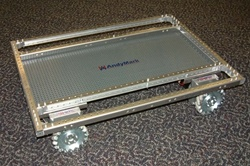
\includegraphics[width=11cm]{pics/chassis/andymark_chassis.jpg}
\end{center}

\subsection{Overview}
\botname's Chassis is the AndyMark C-Chassis with Mecanum Wheel Drive. This chassis was chosen among others because of its price, modularity, and size.

\subsection{Assembly}
\subsection{Troubleshooting}
\subsection{References}

\begin{table}[h!]
  \begin{tabular}{| c | c |}
    \hline
    \textbf{AndyMark Frame Assembly} &  http://files.andymark.com/am-0952AssemblyInstructions.pdf\\
    \hline
    \textbf{AndyMark Gearbox Assembly} &  http://files.andymark.com/x2010-toughbox-user-guide.pdf\\
    \hline
  \end{tabular}
  \label{tab:fire_cmd_msg}
\end{table}

\section{T-Shirt Cannon}
\begin{center}
    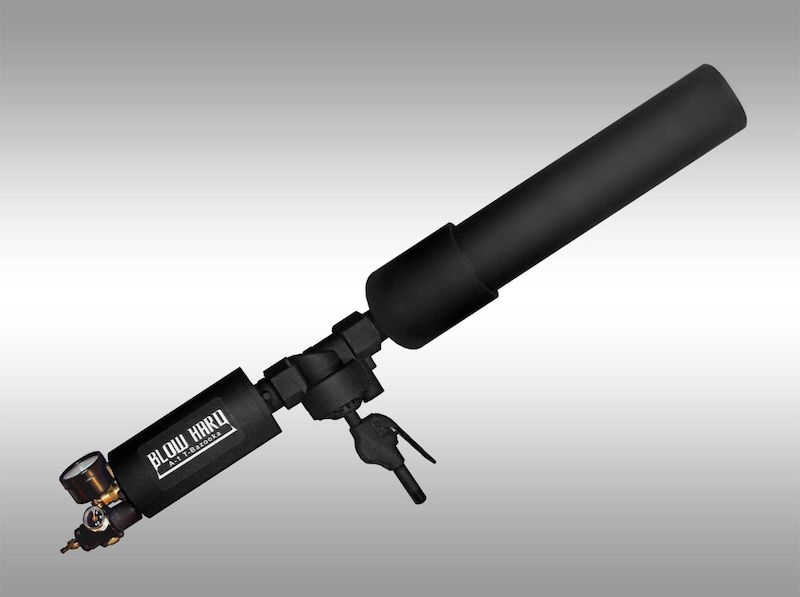
\includegraphics[width=11cm]{pics/cannon/blowhard_cannon.jpg}
\end{center}

\subsection{Troubleshooting}
\begin{center}
    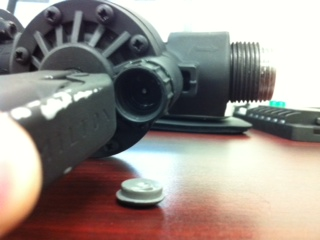
\includegraphics[width=11cm]{pics/cannon/broken_release_valve.jpg}
\end{center}


\end{document}
